\documentclass[12pt, aspectratio=169, xcolor={table}]{beamer}
\usetheme{Copenhagen}
\usecolortheme{beaver}
\setbeamertemplate{navigation symbols}{}

\usepackage{lipsum}

\author{Peter Orosz}
\title{Beamer Practice}
\institute{University of Miskolc}
\date{2022.10.25.}

\begin{document}
	\section{Exercises 1}
	\begin{frame}{Table of Contents}
		\tableofcontents[currentsection]
	\end{frame}
	\subsection{Make Title}
	\begin{frame}
		\maketitle
	\end{frame}
	\subsection{Frame Sub Title}
	\begin{frame}{1st Frame}{1st Frame Sub Title}
		
	\end{frame}
	\subsection{Verbatim}
	\begin{frame}[fragile]{2nd Frame}
		\begin{verbatim}
			This is a \begin{verbatim} environment.
		\end{verbatim}
	\end{frame}
	\subsection{Frame Breaks}
	\begin{frame}[allowframebreaks]{3rd Frame}
		\lipsum[1]\\
		\lipsum[1]\\
		\lipsum[1]\\
		\lipsum[1]\\
	\end{frame}
	\section{Exercise 2}
	\begin{frame}{Table of Contents}
		\tableofcontents[currentsection]
	\end{frame}
	\subsection{Columns}
	\begin{frame}{4th Frame}
		\begin{columns}
			\begin{column}{0.5\linewidth}
				\transduration{2}
				\begin{itemize}
					\item List 1
					\item List 2
					\item List 3
				\end{itemize}
				\begin{enumerate}
					\item Enum 1
					\item Enum 2
					\item Enum 3
				\end{enumerate}
			\end{column}
			\begin{column}{0.5\linewidth}
				\begin{figure}
    				\centering
    				\textbf{Duck}\par\medskip
    				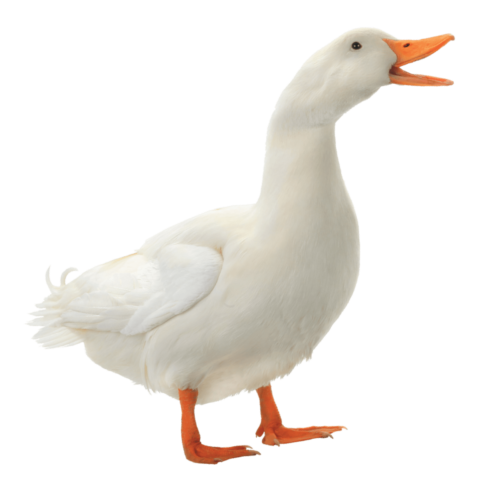
\includegraphics[scale=0.3]{example-image.png}
				\end{figure}
			\end{column}
		\end{columns}
	\end{frame}
	\subsection{Blocks}
	\begin{frame}{5th Frame}
		\begin{block}{Block}
			This is a Block!
		\end{block}
		\pause
		\begin{exampleblock}{Example Block}
			This is an Example Block!
		\end{exampleblock}
		\pause
		\begin{alertblock}{Alert Block}
			This is an Alert Block!
		\end{alertblock}
	\end{frame}
	\subsection{Theorem}
	\begin{frame}{6th Frame}
		\begin{theorem}
			This is a theorem!
		\end{theorem}
		\pause
		\begin{proof}
			This is a proof!
		\end{proof}
	\end{frame}
	\subsection{Semiverbatim}
	\begin{frame}[fragile]{7th Frame}
		\begin{semiverbatim}
			\textcolor{red}{\\begin\{itemize\}}
				\textcolor{green}{\\item Item 1}
				\textcolor{green}{\\item Item 2}
					\textcolor{blue}{\\begin\{itemize\}}
						\textcolor{purple}{\\item Sub Item 1}
						\textcolor{purple}{\\item Sub Item 2}
					\textcolor{blue}{\\end\{itemize\}}
				\textcolor{green}{\\item Item 3}
			\textcolor{red}{\\end\{itemize\}}
		\end{semiverbatim}
	\end{frame}
	\begin{frame}{8th Frame}
		\only<1>{
			\begin{figure}
    			\centering
    			\textbf{Duck 1}\par\medskip
    			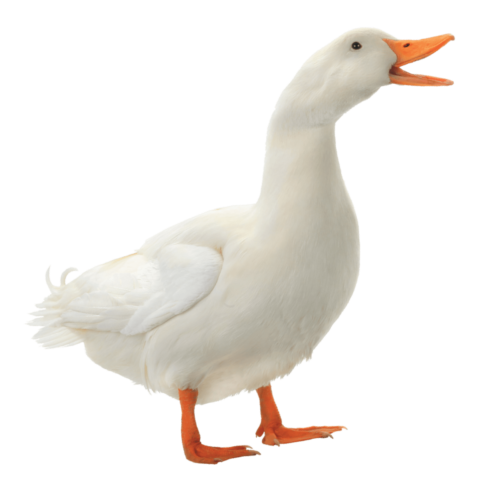
\includegraphics[height = 0.5\textheight]{example-image.png}
			\end{figure}
		}
		\transdissolve<2>
		\only<2>{
			\begin{figure}
    			\centering
    			\textbf{Duck 2}\par\medskip
    			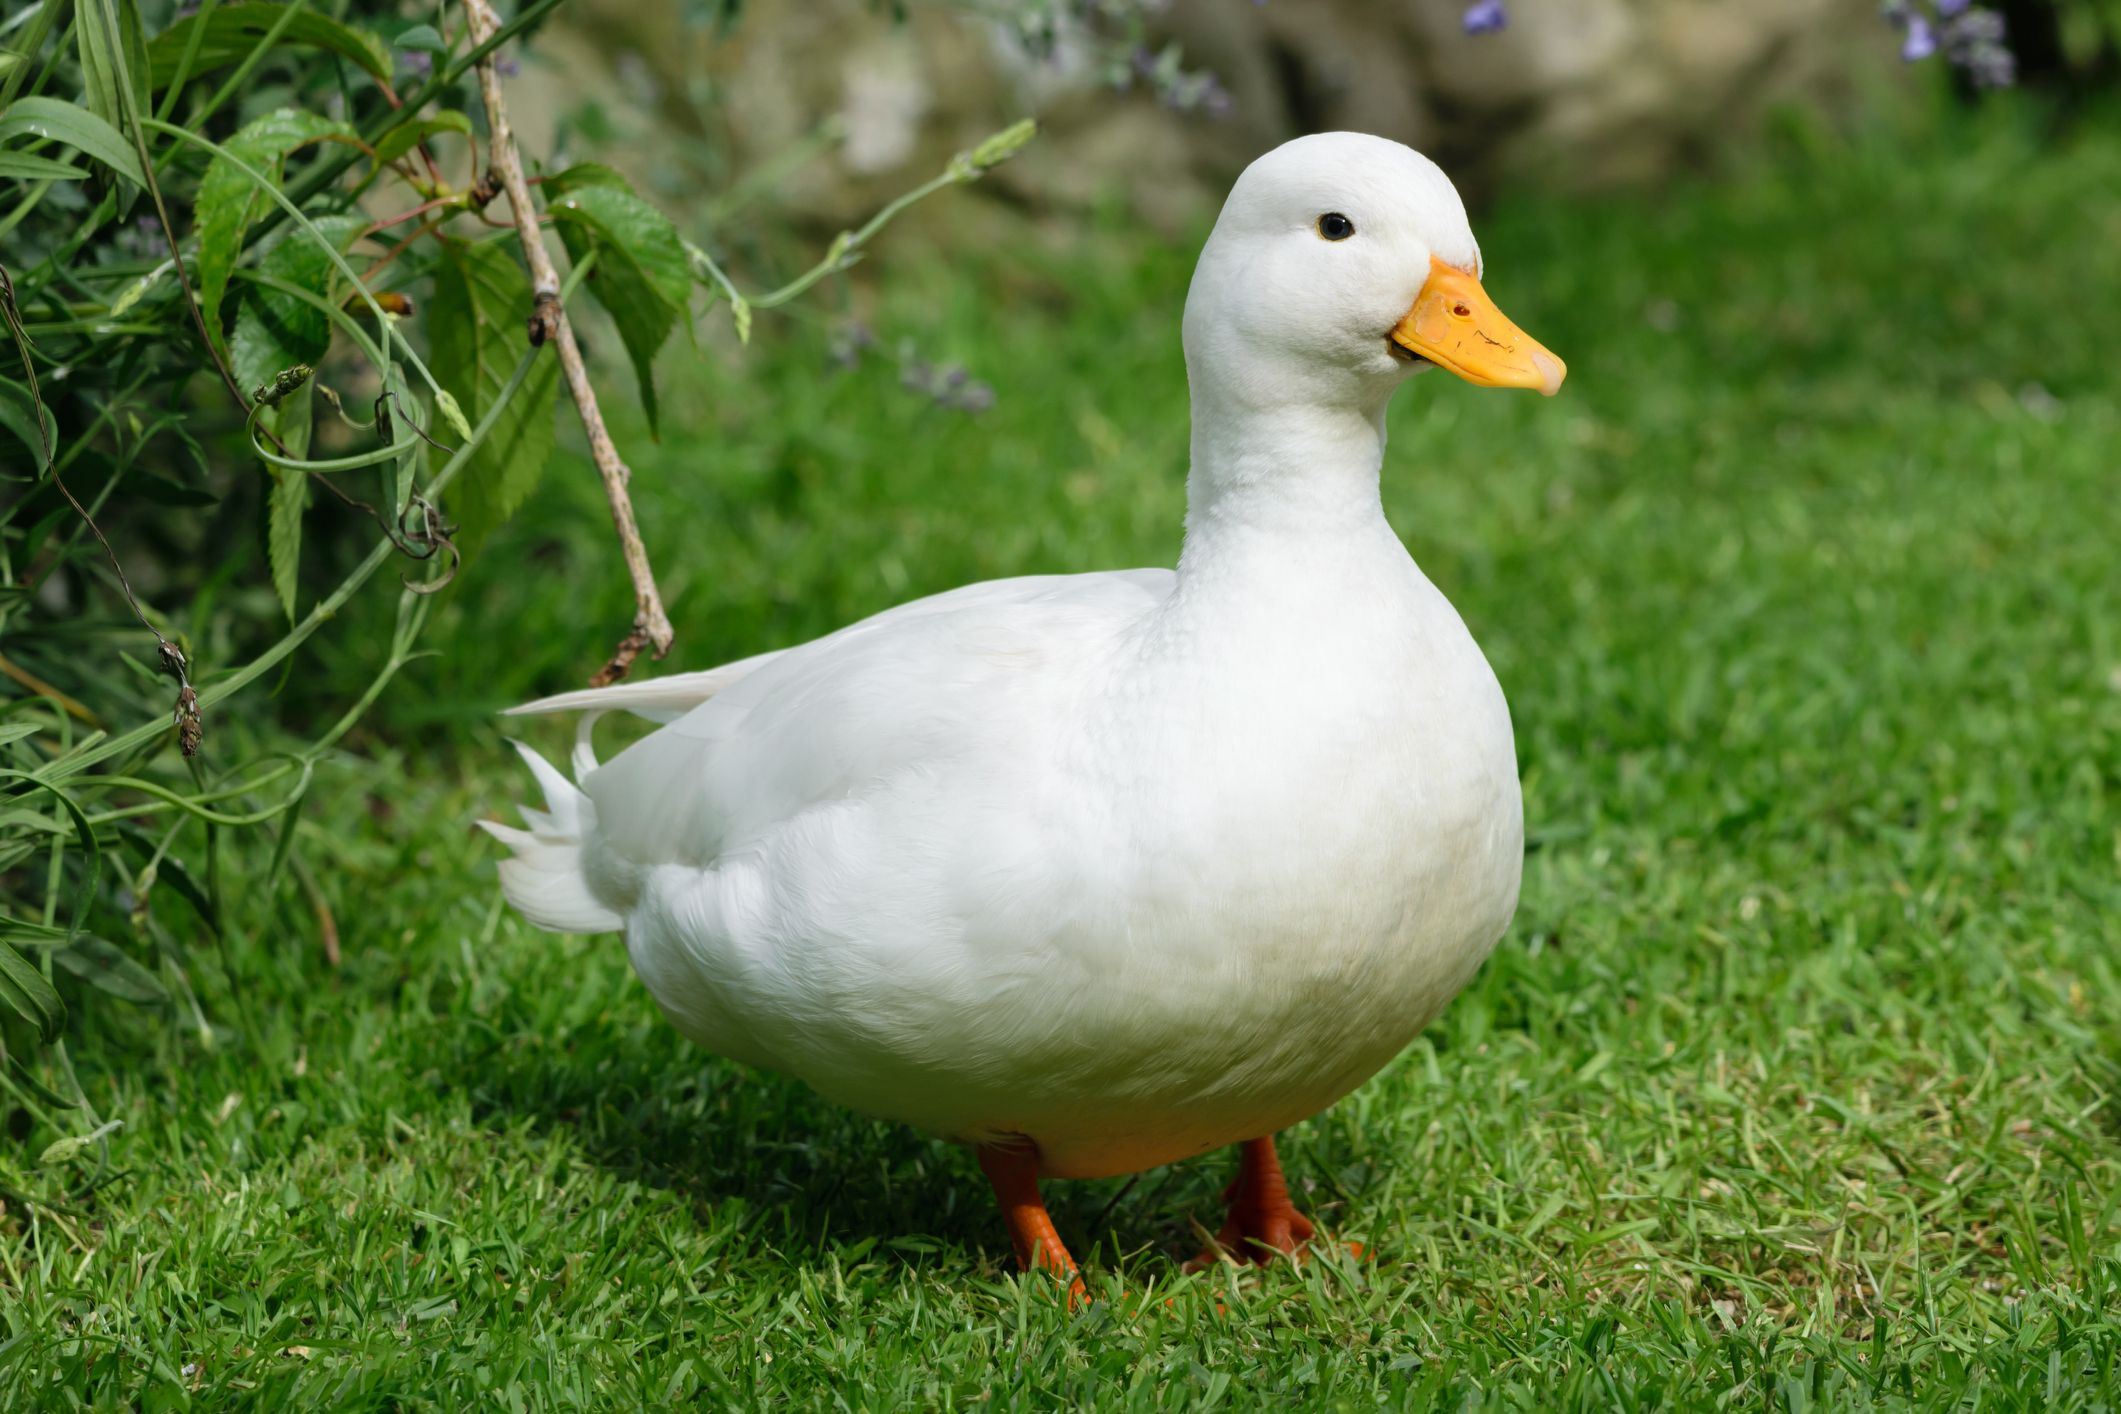
\includegraphics[height = 0.5\textheight]{example-image2.jpg}
			\end{figure}
		}
	\end{frame}
\end{document}